\documentclass[master]{outhesis}

\title{Nurturing as Safe Exploration Promotes the Evolution of Generalized Supervised Learning}
\author{Bryan Hoke}
\degreename{Master of Science}
\school{School of Computer Science}
\chair{Dr. Dean Hougen}
\readerA{Dr. Amy McGovern}
\readerB{Dr. Ingo Schlupp}
\abstractfile{Abstract.tex}

\usepackage{amsmath}
\usepackage{graphicx}
\usepackage{float}
\usepackage[round,authoryear]{natbib}

\graphicspath{ {Figures/} }

\newcommand{\mutationrate}{0.1}
\newcommand{\crossoverrate}{0.8}
\newcommand{\populationsize}{40}
\newcommand{\learningrulesize}{35}

\begin{document}
\makefrontmatter

% Introduction
\chapter{Introduction}

\citet{Chalmers:1990aa} demonstrated that evolutionary processes can produce artificial systems that learn.
The learning that emerged could be either specific to certain tasks or generalized for any task in the problem space.
It was also possible that learning might not emerge if none of the behavior adjustment rules evolved performed better than adjusting behavior randomly.

In Chalmers's work, learning was the only viable phenotypic strategy that could emerge from evolution.
However, if other strategies, such as ``instinctual" behavioral responses (i.e., responses that are innate), were able to emerge alongside the strategy of learning, it might be found that learning is not always the strategy that emerges from evolution.
Presumably, the evolutionary environment (or objective function) would have the effect of influencing which strategies emerge; after all, it is reasonable to think that no one strategy would always be optimal for every possible kind of environment. % TODO: Check writing style

A disadvantage of learning is that individuals tend to have low fitness early in their life before they have had the opportunity to learn correct behavior.
This is in contrast to individuals that exhibit instinctive behavior and have high fitness at the start of life.
Such effects could make it less likely for learning to evolve in favor of instinctual behavior.

However, if the penalties incurred during the early stages of learning could be mitigated then learning may be more likely to evolve.
In the biological world this can be observed in the form of nurturing, often from a parent to a child.
In this way, nurturing may increase the competitive viability of learning by protecting the learner from otherwise costly errors made before proper behavior has been acquired \citep{Woehrer:2012aa}.
                                                                                                                                    
This work examines whether learning is less likely to evolve when both instincts and learning have the potential to emerge,
and how the introduction into the environment of a ``nurturing" condition---where mistakes made during learning are not penalized---influences the evolution of learning as opposed to an instinctual strategy where behavior is fixed during an individual's lifetime.
% TODO: Footnote that instincts will be operationally defined later

To explore these questions, this work uses a combination of genetic algorithms and artificial neurons applied to a set of supervised learning tasks (the same tasks, in fact, that were used by Chalmers). The rest of this chapter introduces the following topics, in turn: genetic algorithms, artificial neurons, artificial neural networks, neuroevolution, the evolution of learning, and nurturing.

%% Genetic Algorithms
\section{Genetic Algorithms}

Genetic algorithms were developed by \citet{Holland:1975aa} to explore using artificial evolution as an optimization process.
Many others have built on and applied Holland's ideas for genetic algorithms over the intervening decades,
and several other forms of evolutionary computation have since been developed \citep{Engelbrecht:2007aa}.
What follows in this section is a brief explanation of one typical version of a genetic algorithm that focuses on the mechanisms used in this thesis,
but it should be noted that many other variations exist.

\emph{Genetic algorithms} are a class of search algorithms inspired by the process of evolution by natural selection.
Solutions to a problem are encoded in strings referred to as \emph{chromosomes}.
The distinct variables in the solution representation are encoded in substrings of the chromosome referred to as \emph{genes}.

The procedure begins with a population of chromosomes which are typically randomly generated.
The chromosomes are evaluated by an objective function---the problem to be solved---referred to as the \emph{fitness function} to determine the fitness value of each one.
The goal of the genetic algorithm is to find the chromosome which maximizes the fitness function and has the highest fitness;
in this sense, a genetic algorithm can be used as a search algorithm that looks for the best solution for an objective function.

A process of selection is used to determine the chromosomes which will reproduce into the next generation based on their fitness values,
 where individuals with higher fitness are more likely to be selected.
 In \emph{roulette-wheel selection}, individuals are selected with a probability that is linearly proportional to their fitness.
 In \emph{elitist selection}, the individual with the highest fitness is automatically selected.

The selection chromosomes then reproduce to create the next-generation population.
One operation used in reproduction is \emph{crossover}, where segments of two chromosomes are combined to create a new chromosome.
The offspring chromosomes may also undergo a process of \emph{mutation}, where each gene has its value changed with some probability, in order to explore the problem space. 

This process is repeated until some stopping condition is met, typically after a certain number of generations.

% TODO: Rotate and/or reduce the size of this figure so it takes up at most 1/3 of the page
\begin{figure}[H]
	\centering
	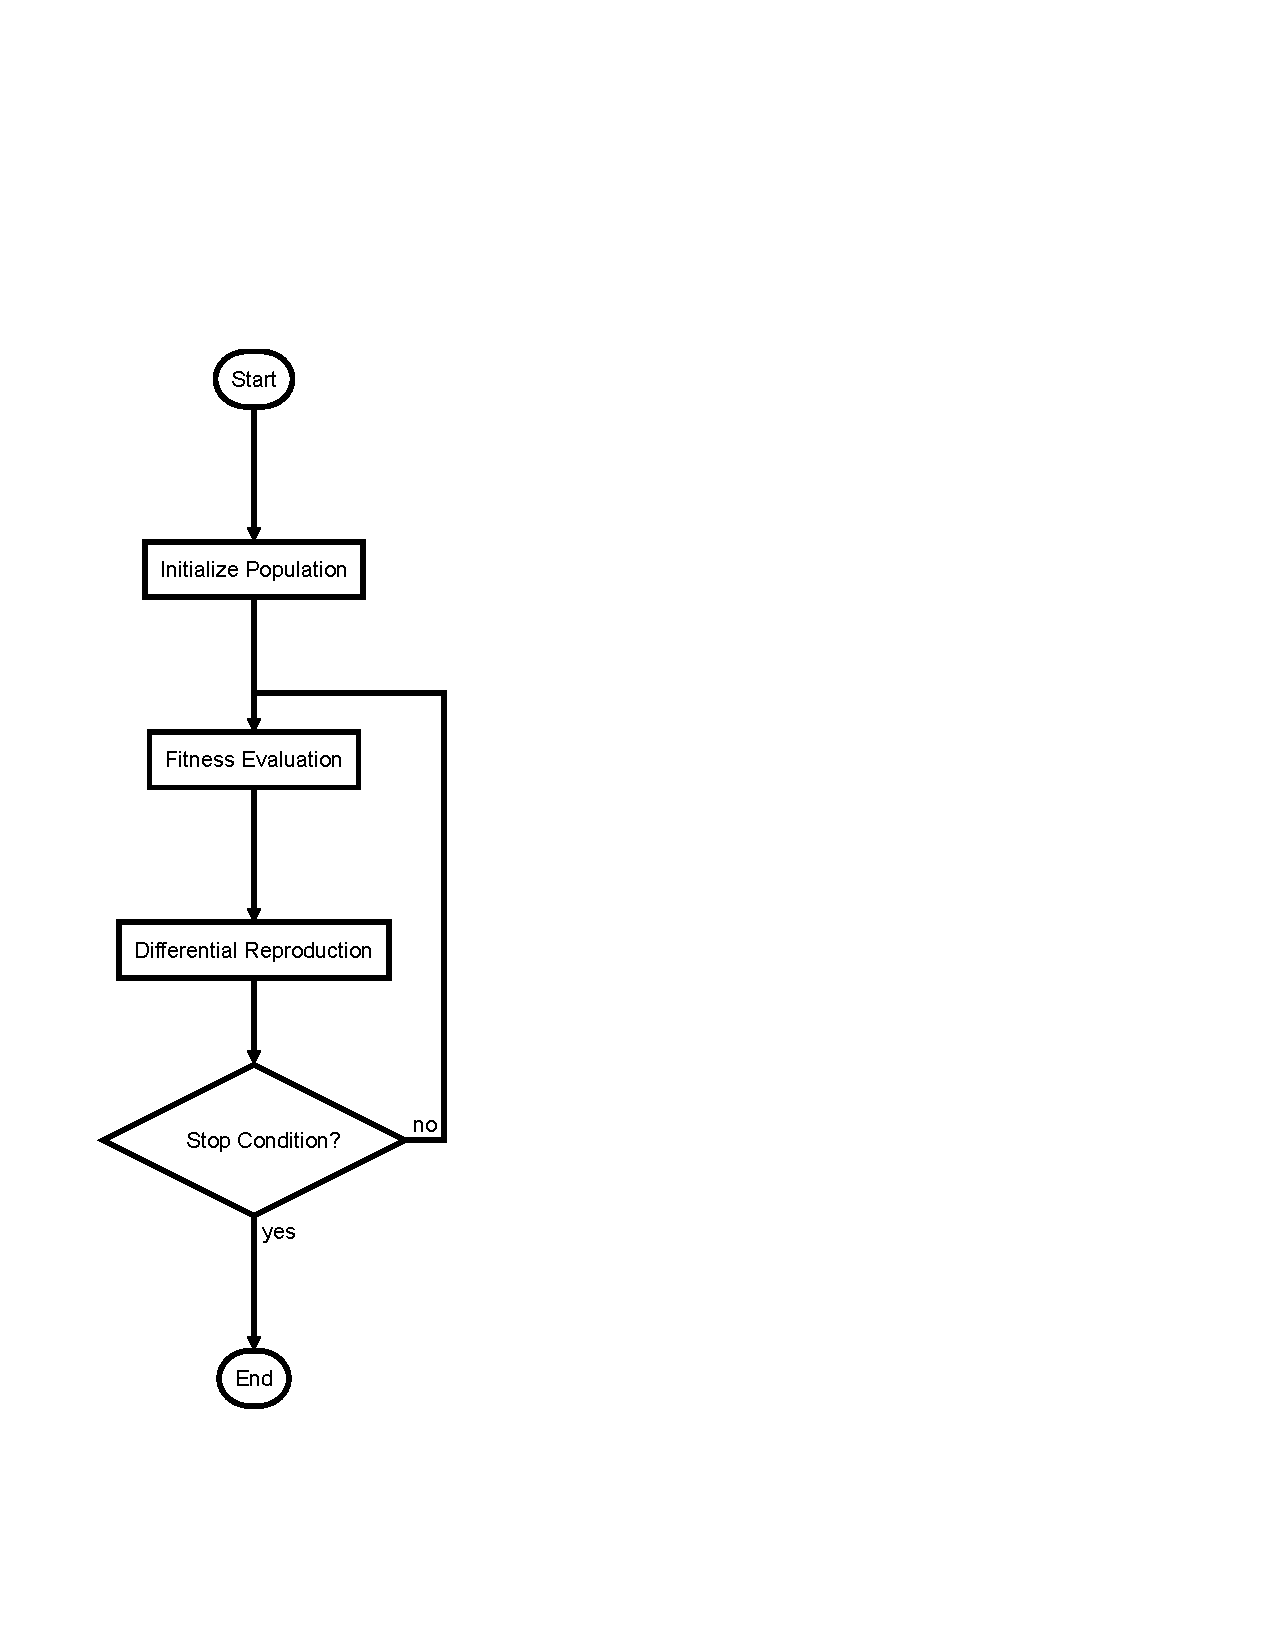
\includegraphics{GeneticAlgorithm.pdf}
	\caption{A high-level view of a genetic algorithm.}
\end{figure}

%% Artificial Neurons
\section{Artificial Neurons}

The concept of an artificial neuron was introduced first by \citet{McCulloch:1943aa} as a theoretical model of biological nervous activity.
Many others have expanded upon this neural model and have developed a number of different neural models \citep{Engelbrecht:2007aa}.
What follows in this section is a brief explanation of one typical version of an artificial neuron that focuses on the mechanisms used in this thesis,
but it should be noted that many other variations exist.

Artificial neurons are computational elements inspired by the biological neurons found in nature.
An artificial neuron is comprised of a number of weighted input connections, an activation function which implements a response to input, and a number of output connections.

% TODO: Match the font in this figure to the font in the text
\begin{figure}[H]
	\centering
	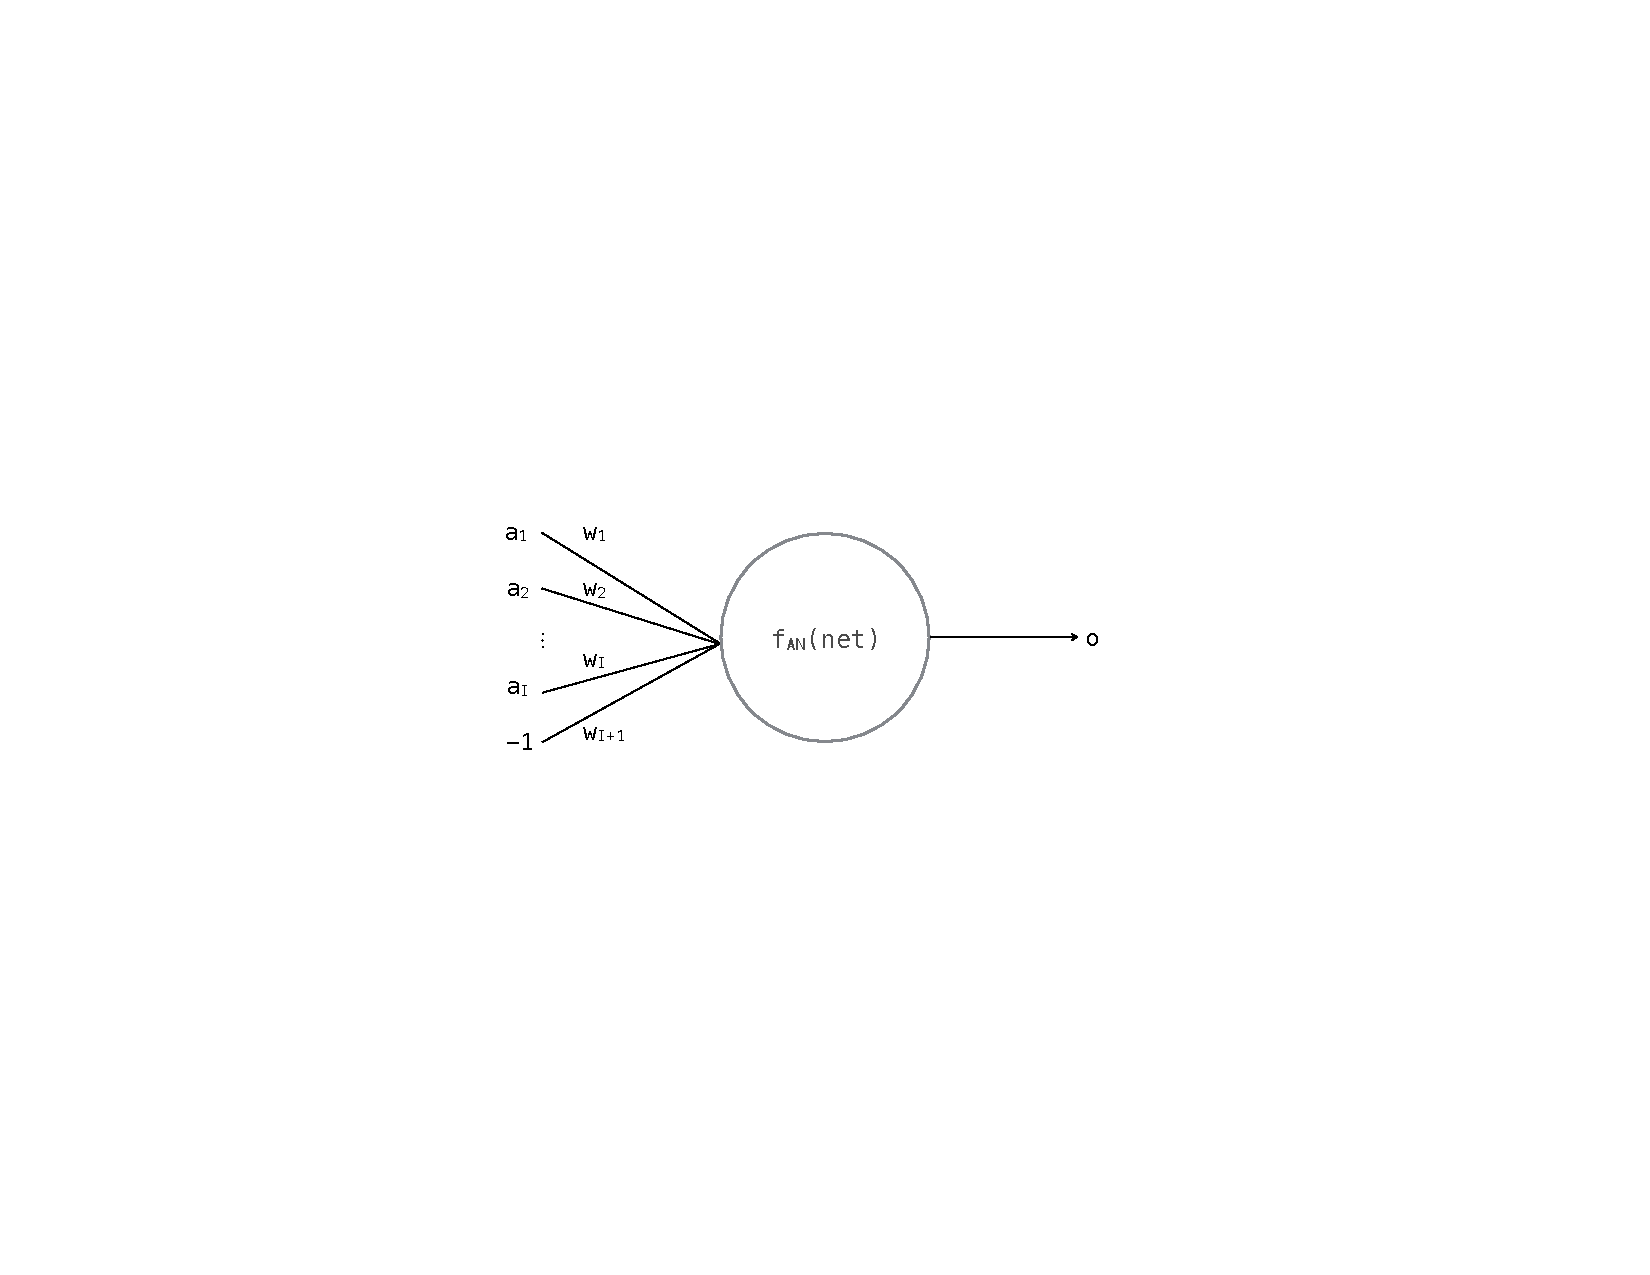
\includegraphics{ArtificialNeuron.pdf}
	\caption{An artificial neuron.}
	\label{fig:neuron}
\end{figure}

Figure \ref{fig:neuron} depicts an artificial neuron with $I$ inputs, one output, and an activation function $f_{AN}$. The neuron receives a vector of $I+1$ input signals, $\mathbf{a}=(a_1, a_2, \ldots, a_I, a_{I+1})$, where $a_{I+1}$ is known as a \emph{bias unit} and always has a value of $-1$.  The input vector is modulated by a weight vector, $\mathbf{w}=(w_1, w_2, \ldots, w_I, w_{I+1})$, where each weight $w_i$ modulates the input signal $a_i$. The neuron computes the net input as the sum of the weighted input signals, giving
\begin{displaymath}
net=\sum_{i=1}^{I+1}a_iw_i.
\end{displaymath}
The output signal, $o$, is then computed by applying the activation function to the weighted input, so that $o=f_{AN}(net)$.

A common choice for $f_{AN}$ is the sigmoid function:

\begin{displaymath}
f_{AN}(net) = \frac{1}{1 + e^{-\lambda net}}
\end{displaymath}
where the parameter $\lambda$ influences the steepness of the function, but usually $\lambda = 1$.

Artificial neurons can be used to compute linearly separable functions without error. This means that, for such a function, there exists at least one threshold value such that the neuron can separate the space of $I$-dimensional input vectors which produce an above-threshold output from those which produce a below-threshold output by an $I$-dimensional hyperplane. This threshold is determined by the bias weight $w_{I+1}$, meaning that the neuron can be used to separate the input vectors for which $net > 0$ from the input vectors for which $net \le 0$.

Learning is a technique by which the weights of an artificial neuron are updated to realize functions given by data.
One type of learning is known as \emph{supervised learning}, where the neuron is provided with a data set, known as the \emph{training set}, consisting of training patterns of input vectors with associated target outputs.
The weights of the neuron are then adjusted until the error between the actual outputs of the neuron and the target outputs in the patterns is minimized.

An example of a supervised learning rule is the so-called \emph{delta rule} \citep{Widrow:1960aa}.
The delta rule requires the definition of an error function, $\mathcal{E}$, to measure the neuron's error in approximating training targets.
The sum of squared errors is usually used, given by

\begin{displaymath}
\mathcal{E} = \sum_{p=1}^{P_T}(t_p-o_p)^2
\end{displaymath}
where $t_p$ and $o_p$ are the target and actual output for the $p$th pattern, and $P_T$ is the total number of patterns in the training set.

Given a single training pattern, weights are updated using

\begin{displaymath}
w_i(t) = w_i(t - 1) + \Delta w_i(t)
\end{displaymath}
with
\begin{displaymath}
\Delta w_i(t) = \eta(- \frac{\partial \mathcal{E}}{\partial w_i})
\end{displaymath}
where
\begin{displaymath}
\frac{\partial \mathcal{E}}{\partial w_i} = -2(t_p - o_p)\frac{\partial f_{AN}}{\partial net_p}a_{i,p}
\end{displaymath}
and $\eta$ is a constant known as the learning rate, $net_p$ is the net input for pattern $p$, and $a_{i,p}$ is the $i$th input signal in pattern $p$.

The delta rule requires that its activation function $f_{AN}$ is continuous and differentiable;
this is so the gradient of the error can be followed toward lower values, giving the direction in which the weights should be updated.
If we use the sigmoid function for $f_{AN}$ then
\begin{displaymath}
\frac{\partial f_{AN}}{\partial net_p} = o_p(1 - o_p)
\end{displaymath}
giving
\begin{displaymath}
\frac{\partial \mathcal{E}}{\partial w_i} = -2(t_p - o_p)o_p(1 - o_p)a_{i,p}
\end{displaymath}

Artificial neurons are generally connected together into artificial neural networks to perform more sophisticated computation;
however, this work is based closely on the work of \citet{Chalmers:1990aa} which considered single neurons in isolation.

%% Artificial Neural Networks
\section{Artificial Neural Networks}

Artificial neural networks were first described by \citet{McCulloch:1943aa} in conjunction with their artificial neuron model,
and the field has been developed by many others in the intervening decades \citep{Engelbrecht:2007aa}.
\citet{Rosenblatt:1958aa} developed the perceptron, an algorithm for pattern recognition and one of the first artificial neural networks to be produced.
\citet{Werbos:1975aa} and \cite{Rumelhart:1986aa} developed the backpropagation algorithm for training multi-layer networks.

Today, deep learning network architectures are used for sophisticated pattern recognition and machine learning tasks \citep{Schmidhuber:2015aa}.
The \emph{Neocognitron} \citep{Fukushima:1980aa} was both the first deep neural network and the first convolutional neural network.
\citet{LeCun:1998aa} later developed \emph{LeNet-5}, a convolutional network that became widely used for recognizing hand-written numbers.
The concept of deep learning was further popularized by \citet{Hinton:2006aa}, who referred to ``learning" for ``deep belief nets."

%% Neuroevolution
\section{Neuroevolution}

Any feature of an artificial neural network, such as topology, connection weights, activation functions, learning rules, and input features, can be subjected to an evolutionary process after being string-encoded \citep{Yao:1999lp}.
However, this work will focus on the evolution of connection weights and learning rules.

The connection weights of a non-learning neuron can be evolved as the fixed response of that neuron to input.
This is analogous to the evolution of instincts or what we think of as ``hard-wired" behavior.

Alternately, the initial connection weights of a learning neuron can be evolved as the initial behavior which will be modified by the neuron's learning rule.
This can be beneficial for evolving passably fit initial behavior that is then fine-tuned by learning
but it can also be the case that the values of the initial weights are not adaptive and weights are evolved that are effectively random.

Learning rules can be evolved stand-alone by applying them to neurons initialized with random weights in the fitness function.
In this situation the values of the initial weights do not matter because the idea is to evolve learning rules that will converge on a solution that is independent of the values of the starting weights.

The initial connection weights and the learning rules that modify them can be evolved simultaneously.
In this situation, instincts, learning, or a combination of both can be evolved depending on the environment.
This work will examine the outcomes of the simultaneous evolution of connection weights and learning rules under different conditions,
whereas Chalmers examined only the possibility of evolving learning rules.

%% The Evolution of Learning
\section{The Evolution of Learning}

Given the wide variety of artificial neural networks developed over the decades,
the necessity of having appropriate learning rules for each,
and the difficulty in determining such rules,
the evolution of learning in artificial neural networks is a topic of great interest to the research community, 
and while many researchers have investigated many different approaches to the evolution of learning,
many open questions still remain \citep{Soltoggio:2017bl}.

Evolution and learning are both forms of adaptation.
Evolution takes place across generations whereas learning takes places within an individual's lifetime.
Evolution can produce adaptive behaviors such as learning or non-adaptive behaviors such as instincts.

If an environment is sufficiently diverse or dynamic, instinctual behavior is not reasonably adequate for good task performance;
this is because such an environment will invariably present novel tasks to which the instinctual behavior is not well-adapted.
Evolved learning behavior that is scalable and adaptive to unknown or changing situations can be seen in countless species in nature.

\citet{Bengio:1990aa} first proposed the optimization of a learning rule via evolutionary search.
\citet{Chalmers:1990aa} evolved learning rules by encoding the parameters of a template formula as strings, demonstrating that the delta rule for supervised learning can be evolved in certain situations for artificial neurons in static environments.
\citet{Fontanari:1991aa} expanded upon Chalmers's approach to evolve a learning algorithm for single-layer networks with binary weights.

% TODO: Say more about the work of both Chalmers and Shaw. 

\citet{McQuesten:1997aa} evolved reinforcement learning by culling subpar individuals and having parent networks teach their offspring using backpropagation.
\citet{Niv:2002aa} demonstrated the evolution of reinforcement learning in uncertain environments for networks with a single binary output.
\citet{Shah:2015hs} similarly demonstrated the evolution of reinforcement learning in changing environments for networks with large numbers of rational-valued outputs.

%% Nurturing
\section{Nurturing}

\emph{Nurturing} is defined as ``the contribution of time, energy, or other resources by one individual to the expected physical, mental, social, or other development of another individual with which it has an ongoing relationship" \citep{Woehrer:2012aa}.

Nurturing is prevalent in the biological world and can be an important contributing factor to the evolution of learning \citep{Woehrer:2012aa,Eskridge:2012aa},
an idea which has recently been echoed by others \citep{Soltoggio:2017bl}.

Nurturing itself can be either instinctive or learned.
\citet{Leonce:2012aa} demonstrated the evolution of instinctive nurturing in robots.

%TODO: Include material here on the virtuous cycle that is hypothesized to exist between nurturing and learning.

Nurturing can cover the initial costs of a learner and the resulting benefits of learning can be paid forward to the next generation.
In this way, nurturing can promote the evolution of learning.

The work of \citet{McQuesten:1997aa},
where it was shown that neuroevolution could benefit from parent networks teaching their offspring using backpropagation,
is the first known example demonstrating that nurturing can promote the evolution of learning;
although McQuesten and Miikkulainen did not refer to the teaching they used as nurturing,
it conforms to the definition followed in this thesis.
\citet{Eskridge:2012aa} conducted experiments involving food patch estimation in uncertain environments,
and their results demonstrated that nurturing as both social learning and safe exploration can promote the evolution of learning.
\citet{Shah:2015hs} demonstrated that nurturing as task simplification can promote the evolution of reinforcement learning in changing environments.

This work explores nurturing as safe exploration in that individuals do not incur fitness penalties for mistakes made during the learning process.

% % Contents of the Thesis
\section{Contents of the Thesis}

The rest of this thesis is organized as follows:
Hypotheses about how nurturing affects the evolution of learning and instincts are detailed in \textbf{Chapter 2}. 
Operational definitions for terms such as ``nurturing" and ``instincts" are introduced in \textbf{Chapter 3}.
Procedures for the experiments examining the effect of nurturing on the evolution of learning and instincts are detailed in \textbf{Chapter 4}.
The experimental results, which demonstrate that nurturing facilitates the evolution of learning, are outlined in \textbf{Chapter 5}. 
The conclusion that nurturing facilitates the evolution of learning is described in \textbf{Chapter 6}. 
Finally, ideas for exploring the interaction between nurturing and the Baldwin effect in future work are described in \textbf{Chapter 7}.

% Hypotheses
\chapter{Hypotheses}

Three factors are considered with respect to their effects on the evolution of learning:
(1) the number of tasks,
(2) the presence or absence of nurturing, and
(3) the possibility of evolving instincts.
Six hypotheses are formulated to explore these factors,
and we consider them in related pairs.
The first pair, which makes predictions about the addition of a non-nurturing condition to Chalmers's experimental setup, is discussed in Section 2.1.
The second pair, which makes predictions about the addition of instincts to the experimental setup used by the first pair, is discussed in Section 2.2.
The third pair, which makes predictions about the effects of the nurturing and non-nurturing conditions on the evolution of instincts and generalized learning, is discussed in Section 2.3.
Finally, appropriate hypothesis tests for these hypotheses are discussed in Section 2.4.

\section{Hypotheses $H_1$ and $H_2$}

The first two hypotheses consider the effects of adding a non-nurturing condition to Chalmers's original model.

Chalmers demonstrated that the quality of evolved generalized learning mechanisms is proportional to the number of tasks in the evolutionary environment. When there are few tasks in the evolutionary environment, high-quality generalized learning is not expected to evolve
because there is no need for evolution to produce learning that is fit for more general contexts;
instead, we would expect specialized learning rules to evolve which happen to perform well in the evolutionary environment.
However, as the number of tasks in the evolutionary environment increases,
the environment becomes too complex for any specialized learning to perform well in,
and so we then expect generalized learning to evolve out of necessity.

Given environments like those used by Chalmers, where instincts cannot be evolved, the addition of nurturing alone is expected to have little impact on the evolution of generalized learning because learning is still the only viable strategy in that setup. Therefore, it is expected that the quality of evolved generalized learning mechanisms will remain proportional to the number of tasks and the quality of the learning evolved will be no greater with nurturing than without.

$\mathbf{H_1}$: When only learning is evolved, the quality of generalized learning evolved will be proportional to the number of tasks in the evolutionary environment, both with and without nurturing.

In other words, we expect to be able both 
to re-confirm Chalmers's conclusion about the evolution of generalized learning
(since the condition under which Chalmers's experiments were performed is effectively the same as the nurturing condition here) 
and to demonstrate that Chalmers's conclusion remains valid even when evaluated under the new non-nurturing condition.

$\mathbf{H_2}$: When only learning is evolved, the quality of generalized learning evolved will be equal with nurturing and without.

This is to say that we do not expect the non-nurturing condition to significantly influence the quality of evolved generalized learning
with respect to the quality of generalized learning evolved under the nurturing condition (i.e., the conditions Chalmers used).
We expect this to be the case because while the non-nurturing condition does make learning less competitive,
there still are no viable alternative strategies to learning that can be evolved.

It is important to note that $H_1$ and $H_2$ are independent hypotheses,
with $H_1$ making a prediction about the effect of varying the number of tasks in the evolutionary environment
and $H_2$ making a prediction about the presence and absence of nurturing.
As such, it is possible for one hypothesis to be supported while the other is not.
For example, 
it could be the case that more complex environments promote the evolution of generalized learning 
but that generalized learning is also less likely to evolve without nurturing because the fitness penalties incurred during learning cause the generalizability of the learning rules evolved to be somewhat compromised by more specialized features that reach higher fitness values more quickly during training (but which perhaps have a lower post-training fitness),
and so the quality of generalized learning evolved is proportional to the number of tasks in the evolutionary environment
but higher-quality generalized learning is evolved with nurturing than without,
in which case $H_1$ would be supported but $H_2$ would not.
Alternately,
it could be the case that the absence of nurturing doesn't affect the quality of generalized learning evolved
but does induce a gating effect on environmental complexity which makes it much more difficult to evolve generalized learning until some threshold complexity is reached,
and so the quality of generalized learning evolved is equal with nurturing and without
but the quality of generalized learning evolved is not linearly proportional to the number of tasks in the evolutionary environment without nurturing,
in which case $H_2$ would be supported but $H_1$ would not. 

\section{Hypotheses $H_3$ and $H_4$}

The introduction of the ability to evolve initial network weights alongside learning rules allows for the evolution of ``instincts" as an alternate strategy to learning. The remaining hypotheses consider the effects of adding the ability to evolve initial network weights to the model developed in the first two hypotheses.

It is expected that higher-quality instincts will evolve for small numbers of evolutionary tasks, but higher-quality learning will evolve as the number of evolutionary tasks increases.
This will be because there will be a smaller number of instinct genes than learning genes to ``tune" to a correct solution for small number of tasks, but because the number of genes required to represent instincts will increase as the number of tasks increases the number of instinct genes will become much larger than the number of learning genes as the number of tasks increases.

$\mathbf{H_3}$: When both instincts and learning are evolved, the quality of instincts evolved will be inversely proportional to the number of tasks in the evolutionary environment, both with and without nurturing.

In other words, higher-quality instincts will evolve with low numbers of tasks in the evolutionary environment,
and lower-quality instincts will evolve with higher numbers of tasks in the evolutionary environment.
We expect this to be the case because the number of genes required to represent instinctive responses to the environment will be proportional to the number of tasks in the environment,
and while it is easy to find good solutions when only small numbers of genes are evolved,
it becomes increasingly difficult to find good solutions as the number of genes involved increases.

$\mathbf{H_4}$: When both instincts and learning are evolved, the quality of generalized learning evolved will be proportional to the number of tasks in the evolutionary environment, both with and without nurturing.

In other words, higher-quality generalized learning will evolve with low numbers of tasks in the evolutionary environment,
and lower-quality generalized learning will evolve with higher numbers of tasks in the evolutionary environment.
We expect this to be the case for the same reasons we expect $H_1$ to be supported;
indeed, $H_4$ can be seen as a prediction that the mechanisms behind $H_1$ will still hold despite the addition of the possibility of evolving instincts.

$H_3$ and $H_4$ can be seen as sort of counterparts to each other 
because they predict that the quality of evolved instincts and generalized learning rules will exhibit opposite trends with respect to the number of tasks in the evolutionary environment; 
that instincts will be strong under the conditions where generalized learning is weak, and vice-versa.
However, it is important to remain clear about the fact that the outcomes of $H_3$ and $H_4$ have no dependencies on each other because they make predictions about instincts and generalized learning with respect to the number of tasks in the evolutionary environment, not each other;
it just so happens that we expect instincts and generalized learning to exhibit opposite trends
but we do not necessarily expect a zero-sum relationship between the two.
For example, it could be the case that learning and instincts are mutually beneficial,
and so the quality of both evolved instincts and generalized learning would be proportional to the number of tasks in the evolutionary environment,
in which case $H_4$ would be supported but $H_3$ would not.
Alternately, it could be the case that
the larger number of genes required for more tasks and the resulting increase in complexity of the search space means that
the quality of both evolved instincts and generalized learning are inversely proportional to the number of tasks in the evolutionary environment,
in which case $H_3$ would be supported but $H_4$ would not.
There are, of course, other possible relationships between the factors involved such that one or the other or both of these hypotheses are false.

\section{Hypotheses $H_5$ and $H_6$}

The final two hypotheses consider the relationship between the nurturing condition (present or absent) and the quality of evolved instincts or generalized learning. Neither of these hypotheses makes a prediction about the relationship between evolved instincts and generalized learning and the number of tasks in the evolutionary environment.

It is expected that higher-quality generalized learning will evolve in the nurturing condition than in the non-nurturing condition because of the costs associated with the learning process in the non-nurturing condition; individuals tend to have low fitness early in their life before they have had the opportunity to learn correct behavior, but in the nurturing condition individuals do not incur fitness penalties for mistakes made early in life.
Likewise, it is expected that higher-quality instincts will evolve in the non-nurturing condition than in the nurturing condition because, without nurturing, the learning individuals will suffer fitness consequences from their unfit initial behavior, increasing the competitive value of instinctual behavior in the evolutionary environment.

$\mathbf{H_5}$: When both instincts and learning are evolved, higher-quality instincts will evolve without nurturing than with.

$\mathbf{H_6}$: When both instincts and learning are evolved, higher-quality generalized learning will evolve with nurturing than without.

Like $H_3$ and $H_4$, $H_5$ and $H_6$ can be seen as counterparts to each other
because they predict that the quality of evolved instincts and generalized learning rules will exhibit opposite effects with respect to the presence or absence of nurturing.
However, as with $H_3$ and $H_4$, it is important to remain clear about the fact that $H_5$ and $H_6$ have no dependencies on each other because they make predictions about instincts and generalized learning with respect to the presence or absence of nurturing, not each other.
For example, it could be the case that under the nurturing condition the increased competitiveness of learning does not inhibit the evolution of instincts,
and so higher-quality generalized learning would evolve with nurturing than without but the instincts evolved with nurturing would be equal to those evolved without,
in which case $H_6$ would be supported but $H_5$ would not.
Alternately, it could be the case that the penalties incurred during learning under the non-nurturing condition promote the evolution of faster, more effective generalized learning than that which tends to evolve under the nurturing condition,
and so higher-quality generalized learning evolves without nurturing than with,
which in turn promotes the evolution of better instincts in an example of what is known as the \emph{Baldwin effect} \citep{Floreano:2008wv},
in which case $H_5$ would be supported but $H_6$ would not.

\section{Hypothesis Testing}

Hypotheses $H_1$, $H_3$, and $H_4$ make predictions about proportionality, 
and so they will be tested using the Pearson correlation coefficient,
which is a measure of the linear correlation between two variables.
Hypotheses $H_2$, $H_5$, and $H_6$ make predictions about performance under one condition being better than performance under another condition,
and so they will be tested using a randomized ANOVA procedure for comparing performance curves \citep{Piater:1998aa}.

% Operational Definitions
\chapter{Operational Definitions}

An \emph{individual} is a candidate solution to the genetic algorithm's fitness function whose characteristics are represented by a chromosome \citep{Engelbrecht:2007aa}. In this work, individuals are manifest as artificial neurons. 

A \emph{task} is a set of input-output patterns,
where for each pattern in the task an individual is evaluated on its ability to produce the pattern output when activated with the corresponding pattern inputs.

An \emph{environment} is a set of tasks by which individuals are assessed.

An individual's \emph{lifetime} is the period during which it is manifest as an artificial neuron and assessed by the fitness function. Specifically, an individual's lifetime consists of a supervised learning period followed by a final evaluation.

\emph{Instincts} are to be represented by the genetically encoded initial weights of a neuron. The tasks are independent, so there will need to be a separate set of instinct weights for each task.

\emph{Learning} is to be represented by the genetically encoded learning rule that is applied to a neuron throughout its lifetime.

For evolved neurons where both initial weights and learning rules are genetically encoded, instinct quality is measured by removing the learning rule and evaluating the fitness of the neuron in the environment in which it was evolved.
For the same neurons, \emph{learning ability} is measured by replacing the genetically encoded initial weights with random initial weights and evaluating the fitness of the neuron in the environment in which it was evolved; \emph{generalized learning ability} is measured by evaluating the fitness of this instinct-removed neuron in an environment different from the one in which it was evolved.

% Is it clear enough that the supervised learning used involves fitness evaluations? 
By default, an individual's lifetime fitness is the average of all fitness evaluations made during learning---when the individual is prone to making mistakes---and the final fitness evaluation that follows learning; this is the ``non-nurturing" condition.
In the ``nurturing" condition, then, an individual's lifetime fitness is simply the result of the final fitness evaluation taken after the individual has had an opportunity to learn correct behavior.

% Procedure
\chapter{Procedure}

%% Genetic Coding of Learning Mechanisms
\section{Genetic Coding of Learning Mechanisms}

The weight update rule for an artificial neuron needs to be based on the components of that neuron which are, as covered in Section 1.2, $a_j$ the activation of the input unit $j$, $o_i$ the activation of the output unit $i$, $t_i$ the training signal on output unit $i$, and $w_{ij}$ the current value of the connection strength from input $j$ to output $i$.

Following \cite{Chalmers:1990aa}, the genome encodes a function $F$ such that $\Delta w_{ij} = F(a_j, o_i, t_i, w_{ij})$, where $F$ is a linear function of its four parameters and their six pairwise products. Thus $F$ is determined by specifying ten coefficients.

The genome encodes these ten coefficients, as well as an eleventh ``scale" parameter. That is,
\[
	\Delta w_{ij} = k_0(k_1w_{ij}+k_2a_j+k_3o_i+k_4t_i+k_5w_{ij}a_j+k_6w_{ij}o_i+k_7w_{ij}t_{i}+k_8a_jo_i+k_9a_jt_i+k_{10}o_it_i),
\]
where $k_0$ to $k_{10}$ are the encoded coefficients.

The portion of the genome which encodes $\Delta w_{ij}$ consists of 35 bits. The first five bits encode the scale parameter $k_0$ such that it can represent the values $0$, $\pm 1/256$, $\pm 1/128$, ..., $\pm 32$, $\pm 64$, via exponential encoding. The first bit encodes the sign of $k_0$ (0: negative, 1: positive), and the next four bits encode the magnitude. If these four bits are interpreted as an integer $j$ between 0 and 15, we have

\[
	|k_0|=
	\begin{cases}
		0 & \text{if $j = 0$}\\
		2^{j-9} & \text{if $j = 1, ..., 15$.}
	\end{cases}
\]

The other 30 bits encode the other ten coefficients in groups of three. The first bit of each group expresses the sign, and the other two bits express a magnitude of 0, 1, 2, or 4 via a similar exponential encoding. If we interpret these two bits as an integer $j$ between 0 and 3, then

\[
	|k_i|=
	\begin{cases}
		0 & \text{if $j = 0$}\\
		2^{j-1} & \text{if $j = 1, 2, 3$.}
	\end{cases}
\]

%% Genetic Coding of Initial Weights
\section{Genetic Coding of Initial Weights}

Initial weights may be evolved alongside learning rules. It would not be meaningful for each chromosome to encode a single set of weights to be used on all tasks, so instead each chromosome simultaneously encodes a distinct set of weights for each task in the evolutionary environment. The weights to be applied to each evolutionary task are encoded in distinct, consistent regions of each chromosome. 

\newcommand{\bitsperweight}{3}
\newcommand{\jlen}{2}
\newcommand{\jmin}{0}
\newcommand{\jmax}{3}
\newcommand{\exponentshift}{4}

Initial weights are encoded using 3 bits each. The first bit is the sign of the weight, and the other two bits express a magnitude of 0, $\frac{1}{2}$, $1$, or $2$ via an exponential encoding. If we interpret the remaining two bits as an integer $j$ between 0 and 3, then

\[
	|k_i|=
	\begin{cases}
		0 & \text{if $j = 0$}\\
		2^{j-2} & \text{if $j = 1, 2, 3$.}
	\end{cases}
\]

For each task the number of weights encoded is equal to the number of inputs in that task plus one bias weight.

%% Evaluation of Fitness
\section{Evaluation of Fitness}

There are two conditions of evaluation: the ``nurturing" case and the ``non-nurturing" case. During evaluation, each network is first trained for 10 epochs using its learning rule. Following this, the network is evaluated on the same tasks. In the ``nurturing" case the individual's fitness is simply the result of the evaluation, whereas in the ``non-nurturing" case the individual's fitness is the average of evaluation during all training epochs and the final evaluation.

Fitness evaluation for the nurturing case:

(1) Create a network with the appropriate number of input units for the task and a single output unit.

(2) Initialize the connection strengths of the network using the values encoded in the chromosome.

(3) For 10 epochs, cycle through the training exemplars for the task, where for each exemplar:

(3a) propagate input values through the system, yielding output values; then

(3b) adjust the weights of the system according to the formula specified by the weight update rule, on the basis of inputs, output, training signal, and current weights.

(4) At the end of this process, fitness on the task is measured by testing the network on all training exemplars, and dividing the total error by the number of exemplars, and subtracting from 1. This yields a fitness value between 0 and 1.

Fitness evaluation for the non-nurturing case:

(1) Create a network with the appropriate number of input units for the task and a single output unit.

(2) Initialize the connection strengths of the network using the values encoded in the chromosome.

(3) For 10 epochs, cycle through the training exemplars for the task, where for each exemplar:

(3a) test the network on the exemplar and measure the error in the network output; then

(3b) propagate input values through the system, yielding output values, then adjust the weights of the system according to the formula specified by the weight update rule, on the basis of inputs, output, training signal, and current weights.

(4) At the end of this process, test the network on all training exemplars and divide the total error of this test and all tests from step 3a by the total number of tests that occurred, and subtracting from 1. This yields a fitness value between 0 and 1.

Fitness of the chromosome is obtained by evaluating its performance on each of the (typically 20) tasks, and taking the mean fitness over all tasks. In this way every chromosome is assigned a fitness between 0 and 1.

%% Parameters of the Genetic Algorithm
\section{Parameters of the Genetic Algorithm}

% TODO: Describe "segment-wise" crossover used

A fixed population size of 40 is used in all experiments. Following the fitness evaluation process described in Section 4.3, a new population of 40 individuals is created as follows:

(1) Elitist selection is applied, meaning that an exact copy of the individual with the highest fitness in the previous population is inserted into the new population.

(2) Roulette-wheel selection (where an individual's probability of being selected is linearly proportional to its fitness) is used to select 39 individuals from the previous population with replacement (so an individual can be selected more than once), then:

(2a) the first 32 selected individuals are reproduced by gene-wise two-point crossover in pairs to create 32 new individuals which are inserted into the new population;

(2b) the remaining 7 selected individuals are reproduced by cloning to create 7 new individuals which are inserted into the new population.

(3) Each individual in the new population is mutated such that each bit in each chromosome has a 1\% chance of changing.

This cycle of fitness-evaluation and reproduction is repeated for 1000 generations.

%Population size: 40
%Crossover rate: 0.8
%Mutation rate: 0.01
%Elitism factor: 1
%Number of generations: 1000

%% Post-Evolutionary Evaluation
\section{Post-Evolutionary Evaluation}

Before each evolutionary run, 10 tasks are selected at random from the task pool and designated as ``test tasks,"
and up to 20 tasks are selected at random from the remaining 20 tasks and designated as ``evolutionary tasks."
New evolutionary tasks and test tasks are selected for each repetition of an evolutionary run and between evolutionary runs  nurturing condition and non-nurturing condition .
After each evolutionary run, the chromosome with the highest fitness score in the history of the populations in that run is identified.
From this chromosome, the learning rule bits are isolated and evaluated on the test tasks (using both the nurturing and non-nurturing conditions) and the bits encoding the initial weights are isolated and evaluated on the evolutionary tasks.
Each evolutionary run is repeated 30 times.

% Results and Discussion
\chapter{Results and Discussion}

This chapter presents the results of all experiments performed.

%% The Evolution of Learning
\section{The Evolution of Learning}

This section presents the results of experiments where learning rules can be evolved but initial weights cannot, performed under both the nurturing and non-nurturing conditions.
% TODO: Mention random weights

%%% Evolutionary Runs
\subsection{Evolutionary Runs}

\begin{figure}[H]
	\centering
	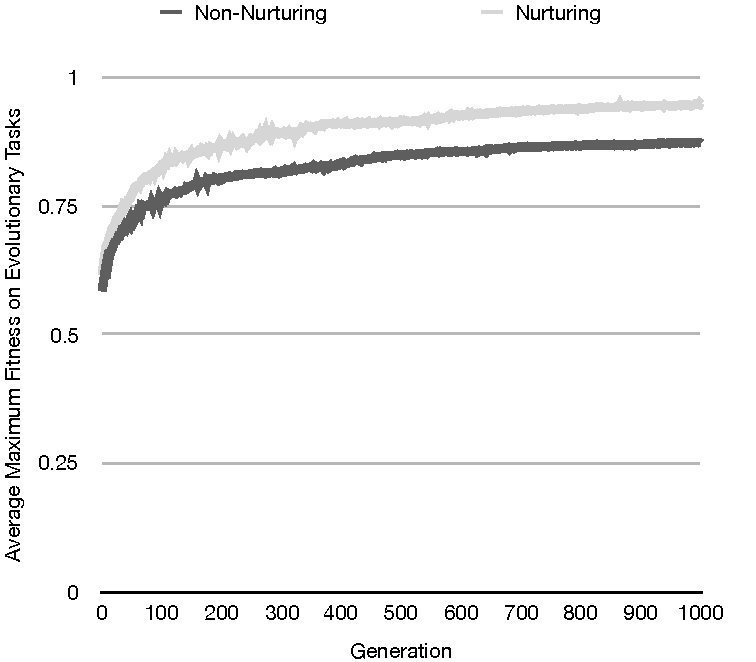
\includegraphics{T1Evolution.pdf}
	\caption{The maximum fitness for populations evolved using 20 tasks under the nurturing and non-nurturing conditions.}
	\label{fig:T1Evolution}
\end{figure}

Figure \ref{fig:T1Evolution} shows the increase of maximum fitness with the progression of generations,
which demonstrates the increasing adaptation of the individuals to their environment.
This is the same trend seen in Figure 1 of \citet{Chalmers:1990aa}, which depicted the evolution of maximum fitness in the populations evolved in that work.
This similarity to previous findings helps to validate our setup as sufficient to observe the evolution of learning
and indicates that we have sufficiently replicated Chalmers's setup to be confident in comparing our results to his.

%%% Generalized Learning Tests
\subsection{Generalized Learning Tests}

\begin{figure}[H]
	\centering
	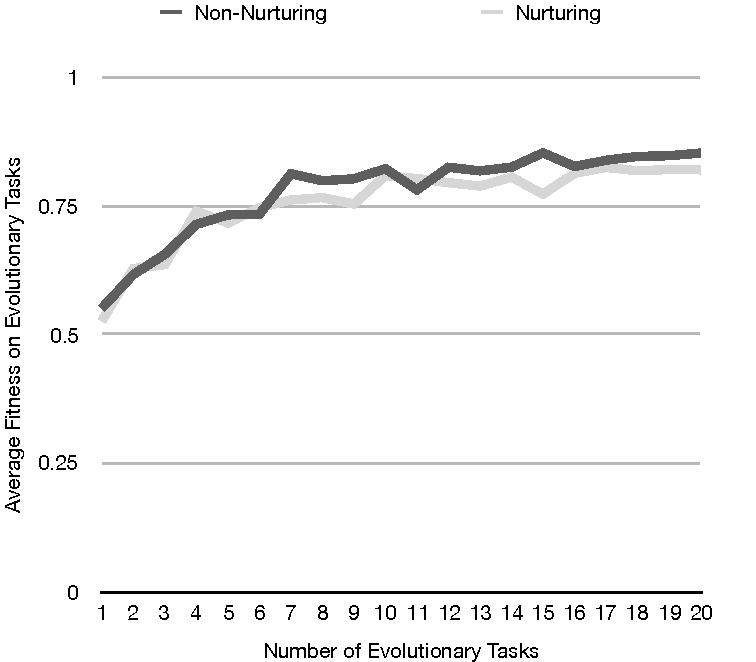
\includegraphics{T1IntraLearningGeneralizationTest.pdf}
	\caption{Intra-learning/non-nurturing generalization test on test tasks for the best individuals evolved under the nurturing and non-nurturing conditions.}
	\label{fig:T1IntraLearningGeneralizationTest}
\end{figure}

\begin{figure}[H]
	\centering
	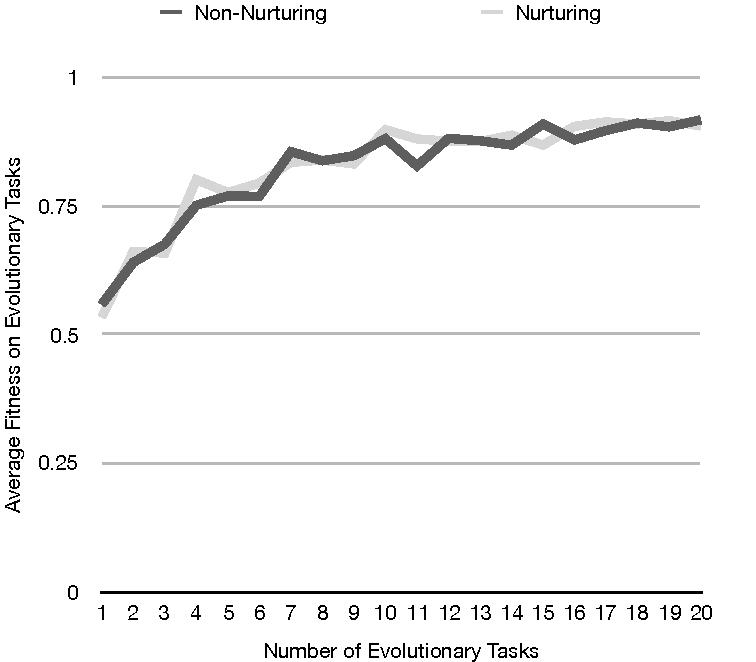
\includegraphics{T1PostLearningGeneralizationTest.pdf}
	\caption{Post-learning/nurturing generalization test on test tasks for the best individuals evolved under the nurturing and non-nurturing conditions.}
	\label{fig:T1PostLearningGeneralizationTest}
\end{figure}

The linear correlation between the intra-learning generalized learning fitness and the number of evolutionary tasks is statistically significant for both
the nurturing condition (Pearson correlation, $\rho=0.61,$ $p < 0.001$)
and the non-nurturing condition (Pearson correlation, $\rho=0.60,$ $p < 0.001$).

The differences between the intra-learning generalization test results for the nurturing and non-nurturing conditions are statistically significant (randomized ANOVA, algorithm $p < 0.001$, interaction $p = 0.0270$).

The linear correlation between the post-learning generalized learning fitness and the number of evolutionary tasks is statistically significant for both
the nurturing condition (Pearson correlation, $\rho=0.63,$ $p < 0.001$)
and the non-nurturing condition (Pearson correlation, $\rho=0.59,$ $p < 0.001$).

The differences between the post-learning generalization test results for the nurturing and non-nurturing conditions are not statistically significant (randomized ANOVA, algorithm $p = 0.2120$, interaction $p = 0.0350$).

Figures \ref{fig:T1IntraLearningGeneralizationTest} and \ref{fig:T1PostLearningGeneralizationTest} demonstrate that the generalized learning capabilities of evolved individuals increases with the number of evolutionary tasks.
This is the same trend shown by the ``Test Fitness" line in Figure 2 of \citet{Chalmers:1990aa}.
Under both evaluation conditions in each test,
the generalized learning fitness was statistically significantly proportional to the number of evolutionary tasks,
suggesting that the quality of evolved generalized learning increases with the number of evolutionary tasks.
This result serves as a re-confirmation of Chalmers's original findings \citep{Chalmers:1990aa}
and shows that they are robust to the change to a non-nurturing condition.

In the post-learning evaluation,
the difference between the quality of generalized learning evolved under the nurturing and non-nurturing conditions was not found to be statistically significant.
This supports our hypothesis that the presence or absence of nurturing will not affect the quality of evolved generalized learning when learning rules can be evolved but initial weights cannot. 

However,
in the intra-learning evaluation,
the learning rule evolved under the non-nurturing condition performed better than the learning rule evolved under the nurturing condition by a statistically significant margin,
suggesting that faster generalized learning is more likely to evolve under the non-nurturing condition.
If ``the quality of generalized learning" is interpreted as including a higher learning rate,
then this could be seen to be contrary to our hypothesis that the presence or absence of nurturing would not affect the quality of evolved generalized learning 
when learning rules could be evolved but initial weights could not.
Nonetheless,
it is important to note that there was no significant difference found in the quality of the learned behaviors at the end of the learning period,
meaning that the higher learning rate is not adaptive under the nurturing condition,
only under the non-nurturing condition.

$\mathbf{H_1}$: When only learning rules are evolved, the quality of generalized learning evolved will be proportional to the number of tasks in the evolutionary environment, both with and without nurturing.

This hypothesis was supported by the results.

$\mathbf{H_2}$: When only learning rules are evolved, the quality of generalized learning evolved will be equal with nurturing and without.

This hypothesis was supported by the results.

%% The Evolution of Learning and Instincts
\section{The Evolution of Learning and Instincts}

This section present the results of experiments where learning rules and initial weights can be evolved, performed under both the nurturing and non-nurturing conditions.

%%% Evolutionary Runs
\subsection{Evolutionary Runs}

\begin{figure}[H]
	\centering
	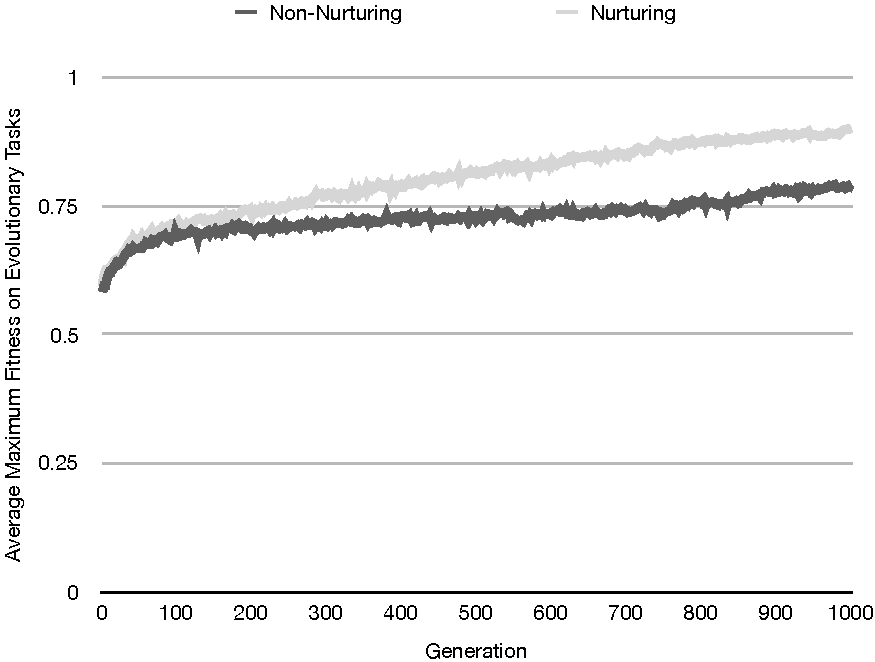
\includegraphics{LearningInstinctsEvolution.pdf}
	\caption{The maximum fitness for populations evolved using 20 evolutionary tasks under the nurturing and non-nurturing conditions.}
	\label{fig:LearningInstinctsEvolution}
\end{figure}

Figure \ref{fig:LearningInstinctsEvolution} shows the increase of maximum fitness with the progression of generations,
which demonstrates the increasing adaptation of the individuals to their environment.
This is the same trend shown by Figure \ref{fig:T1Evolution} and Figure 1 of \citet{Chalmers:1990aa}.
Under both conditions it is clear that the objective function becomes more difficult to satisfy as the number of evolutionary tasks increases. 

%%% Intra-Learning and Post-Learning Fitness Tests
\subsection{Intra-Learning and Post-Learning Fitness Test}

\begin{figure}[H]
	\centering
	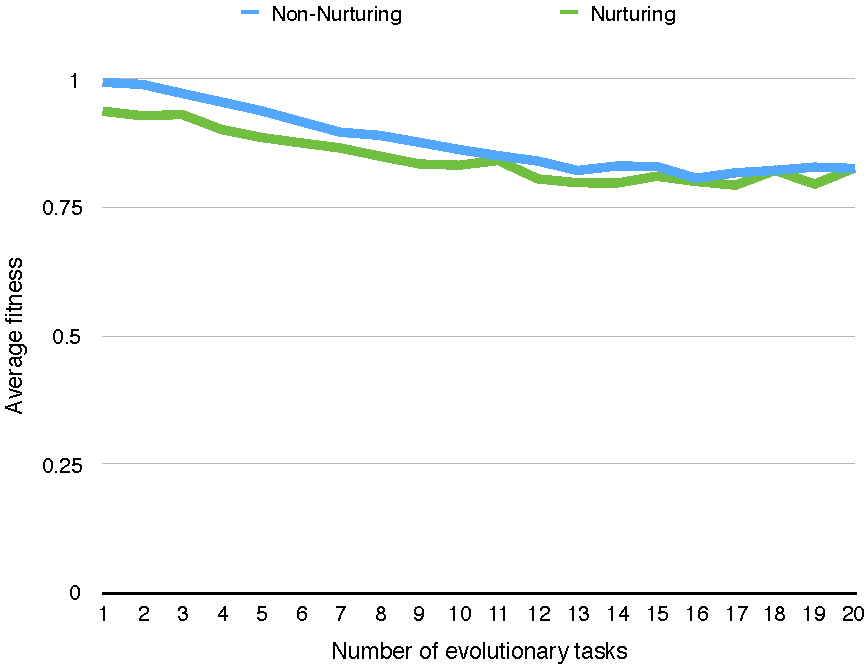
\includegraphics{NonNurturingFitnessTestPlot.pdf}
	\caption{Intra-learning/non-nurturing fitness test on evolutionary tasks for individuals evolved under the nurturing and non-nurturing conditions.}
	\label{fig:T1IntraLearningFitnessTest}
\end{figure}

\begin{figure}[H]
	\centering
	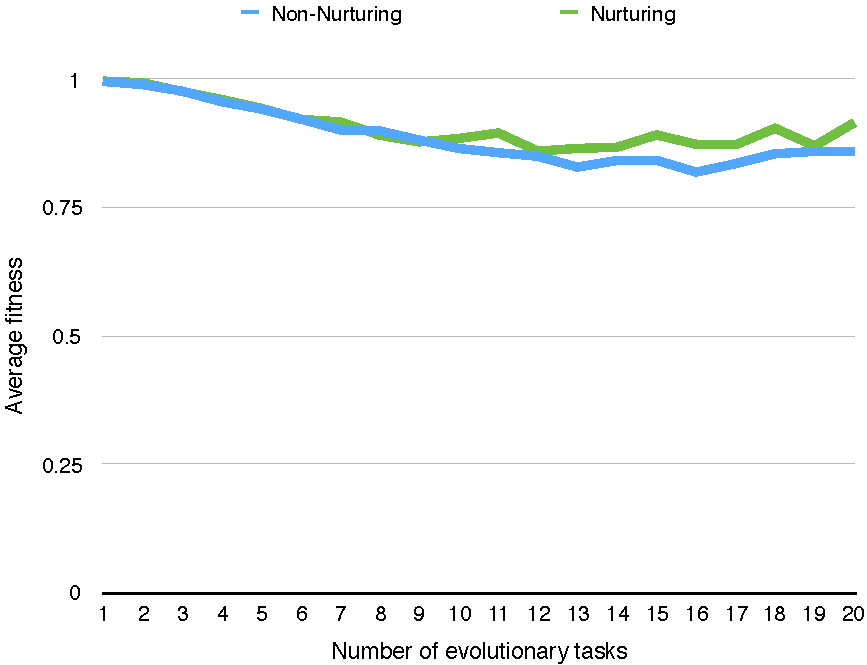
\includegraphics{NurturingFitnessTestPlot.pdf}
	\caption{Post-learning/nurturing fitness test on evolutionary tasks for individuals evolved under the nurturing and non-nurturing conditions.}
	\label{fig:T1PostLearningFitnessTest}
\end{figure}

The individual with the highest fitness in each evolutionary run is re-evaluated on the evolutionary tasks from that run using both the nurturing and non-nurturing conditions (recall that it is evaluated using only one of these conditions during evolution).

The fitness test for the non-nurturing condition can be seen as testing how much fitness an individual would collect on average during the learning process (and one final evaluation immediately afterward);
as such, it will be referred to as the ``intra-learning fitness test."

Similarly, the fitness test for the nurturing condition can be seen as testing how much fitness an individual would collect on average after learning as been completed;
it will be referred to as the ``post-learning fitness test."

The differences between the intra-learning test results for the nurturing and non-nurturing conditions are statistically significant (randomized ANOVA, algorithm $p < 0.0001,$ interaction $p = 0.0090$).

The differences between the post-learning test results for the nurturing and non-nurturing conditions are statistically significant (randomized ANOVA, algorithm $p < 0.0001,$ interaction $p = 0.0220$).

Figures \ref{fig:T1IntraLearningFitnessTest} and \ref{fig:T1PostLearningFitnessTest} show that,
when evaluated using the intra-learning (non-nurturing condition) test,
those individuals evolved under the non-nurturing condition on average outperform those evolved under the nurturing condition,
and when evaluating using the post-learning (nurturing condition) test,
those individuals evolved under the nurturing condition on average outperform those evolved under the non-nurturing condition.
This suggests that the nurturing and non-nurturing conditions present somewhat different criteria for optimal behavior,
and that being very well-adapted adaptation to one condition means being somewhat less well-adapted to the other condition.

%%% Pre-Learning Test
\subsection{Pre-Learning Test}

\begin{figure}[H]
	\centering
	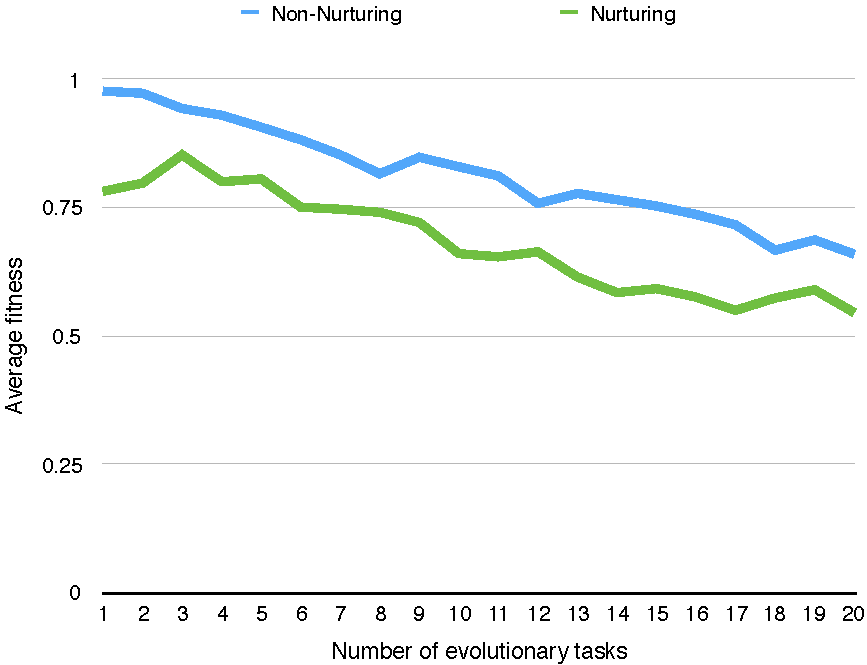
\includegraphics{NetworkTestPlot.pdf}
	\caption{Pre-learning/instinct test on evolutionary tasks for individuals evolved under the nurturing and non-nurturing conditions.}
	\label{fig:PreLearningTest}
\end{figure}

The portion of the chromosome that encodes the initial weights is isolated and evaluated on the evolutionary tasks by initializing a neuron with the encoded weights, 
with the intention of determining the contribution to the fitness of the whole chromosome of just the portion of the chromosome that encodes the initial weights.
In other words, this is intended to test the instincts of the individual in the absence of learning.

The inverse-linear correlation between the pre-learning fitness and the number of evolutionary tasks is statistically significant for both 
the nurturing condition (Pearson correlation, $\rho=-0.63,$ $p < 0.001$)
and the non-nurturing condition (Pearson correlation, $\rho=-0.83,$ $p < 0.001$).

The differences between the results for the nurturing and non-nurturing conditions are statistically significant (randomized ANOVA, algorithm $p < 0.001$, interaction $p < 0.001$).

As shown in Figure \ref{fig:PreLearningTest},
under both evaluation conditions, the pre-learning fitness was statistically significantly inversely proportional to the number of evolutionary tasks,
suggesting that the quality of evolved instincts decreases with the number of evolutionary tasks when it is also possible to evolve learning.

Individuals evolved using the non-nurturing condition performed better on this evaluation than individuals evolved using the nurturing condition by a statistically significant margin,
suggesting that instincts (initial weights) make a larger contribution to fitness in the non-nurturing case than in the nurturing case.

$\mathbf{H_3}$: When both initial weights and learning rules are evolved, the quality of instincts evolved will be inversely proportional to the number of tasks in the evolutionary environment, both with and without nurturing.

This hypothesis was supported by the results.

$\mathbf{H_5}$: When both initial weights and learning rules are evolved, higher-quality instincts will evolve without nurturing than with.

This hypothesis was supported by the results.

%%% Learning Improvement
\subsection{Learning Improvement}

\begin{figure}[H]
	\centering
	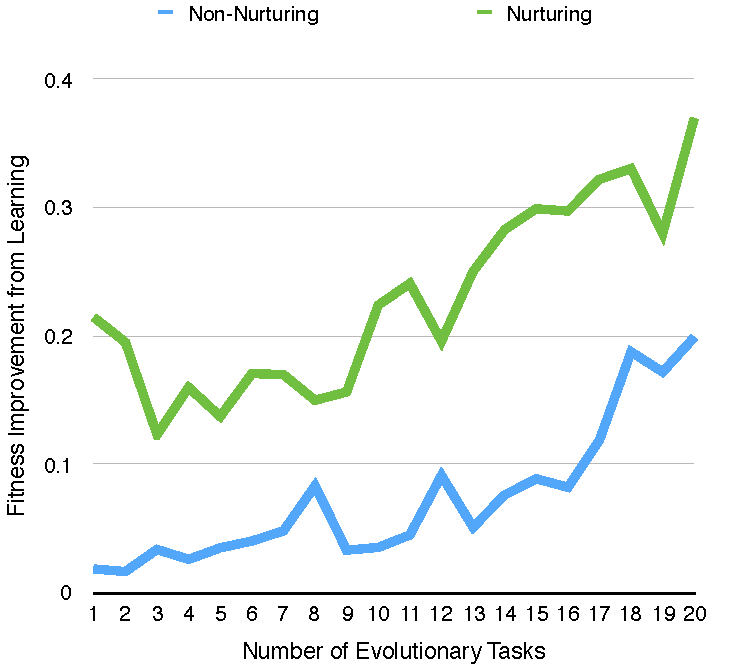
\includegraphics{LearningImprovementPlot.pdf}
	\caption{The difference between evolutionary fitness and network fitness for individuals evolved under the nurturing and non-nurturing conditions.}
	\label{fig:LearningImprovement}
\end{figure}

To determine the average amount of useful learning that evolves for a given number of tasks we can examine the difference between the post-learning fitness and the pre-learning (instinctive) fitness, as shown in Figure \ref{fig:LearningImprovement}.
This is because the pre-learning fitness is the individual's fitness before it learns, whereas the post-learning fitness is an individual's fitness after it learns.

The linear correlation between the learning improvement and the number of evolutionary tasks is statistically significant for both
the nurturing condition (Pearson correlation, $\rho=-0.39,$ $p < 0.001$)
and the non-nurturing condition (Pearson correlation, $\rho=-0.40,$ $p < 0.001$). 

The differences between the results for the nurturing and non-nurturing conditions are statistically significant (randomized ANOVA, algorithm $p < 0.001$, interaction $p < 0.001$).

As shown in Figure \ref{fig:LearningImprovement},
the improvement in fitness due to learning increases as the number of evolutionary tasks increases under both the nurturing and non-nurturing conditions.
This suggests that learning becomes an increasingly important evolutionary strategy as the environment becomes more varied.

%%% Weight-Generalization Learning Test
\subsection{Weight-Generalization Learning Test}

\begin{figure}[H]
	\centering
	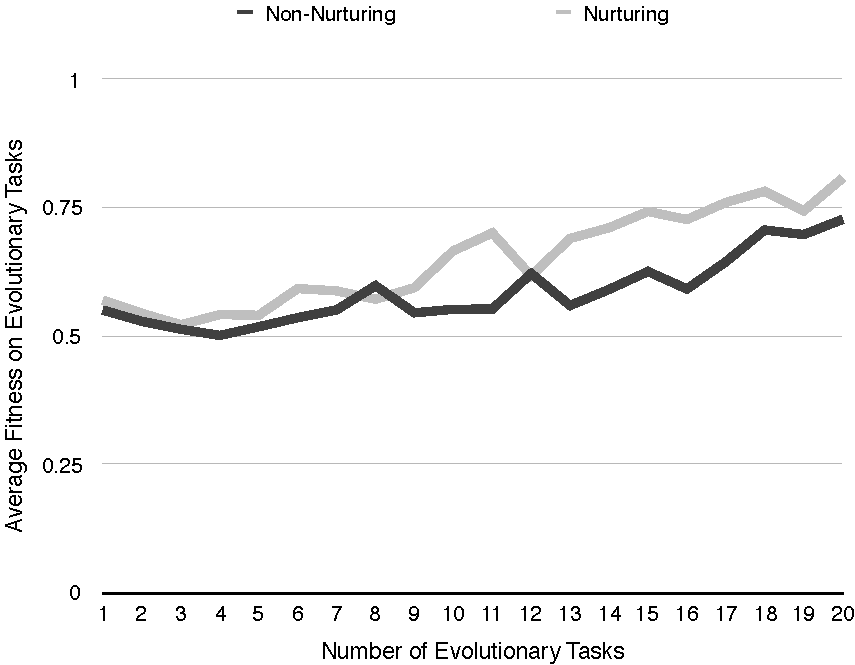
\includegraphics{NonNurturingLearningTestPlot.pdf}
	\caption{Random-start, intra-learning/non-nurturing learning test on evolutionary tasks for individuals evolved under the nurturing and non-nurturing conditions.}
	\label{fig:IntraLearningWeightGeneralizationTest}
\end{figure}

\begin{figure}[H]
	\centering
	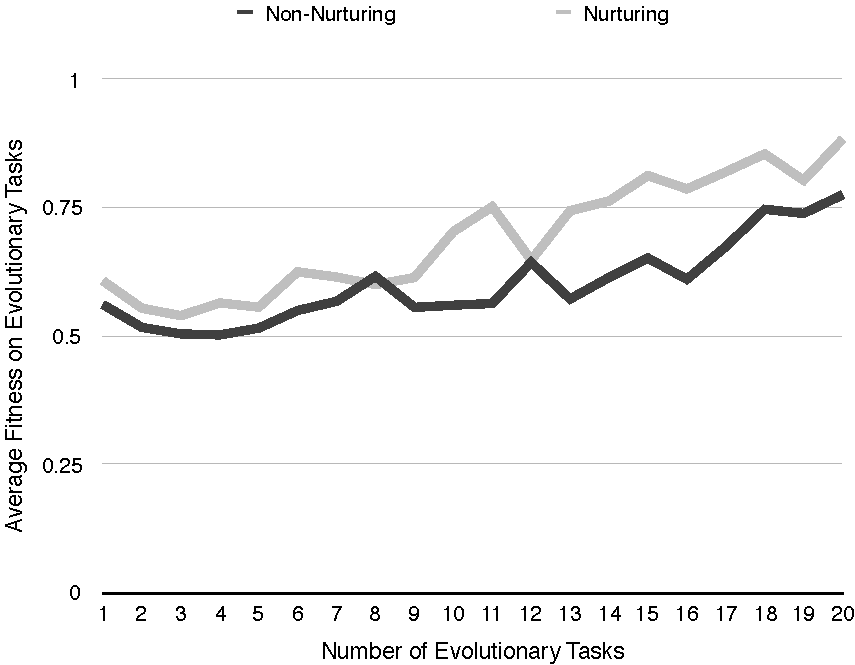
\includegraphics{NurturingLearningTestPlot.pdf}
	\caption{Random-start, post-learning/nurturing learning test on evolutionary tasks for individuals evolved under the nurturing and non-nurturing conditions.}
	\label{fig:PostLearningWeightGeneralizationTest}
\end{figure}

The portion of the chromosome that encodes the learning rule is isolated and evaluated on the evolutionary tasks by initializing a network with random weights and the encoded learning rule, with the intention of determining the contribution of the portion of the chromosome that encodes the learning rule to the fitness of the whole chromosome.

The differences between the intra-learning test results for the nurturing and non-nurturing conditions are statistically significant (randomized ANOVA, algorithm $p < 0.0001,$ interaction $p < 0.0001$).

The differences between the post-learning test results for the nurturing and non-nurturing conditions are statistically significant (randomized ANOVA, algorithm $p < 0.0001,$ interaction $p < 0.0001$).

As shown in Figures \ref{fig:IntraLearningWeightGeneralizationTest} and \ref{fig:PostLearningWeightGeneralizationTest},
the learning rule evolved under the nurturing condition performed better than the learning rule evolved under the non-nurturing condition
when using both the intra-learning and post-learning tests,
suggesting that the learning rule makes a larger contribution to fitness under the nurturing condition than it does under the non-nurturing condition.

%%% Task Generalization Learning Test
\subsection{Task Generalization Learning Test}

\begin{figure}[H]
	\centering
	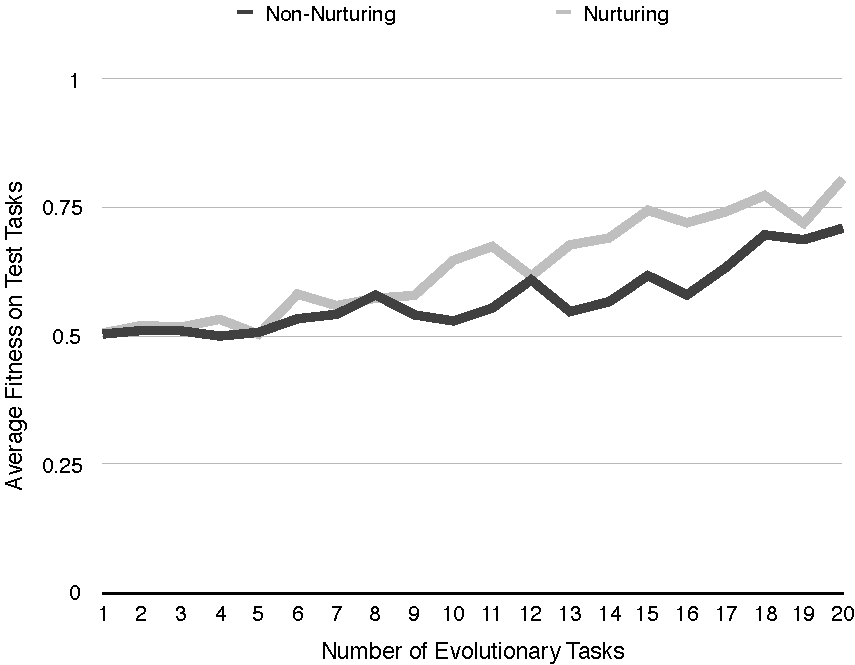
\includegraphics{NonNurturingGeneralizationTestPlot.pdf}
	\caption{Intra-learning/non-nurturing generalization test on test tasks for individuals evolved under the nurturing and non-nurturing conditions.}
\end{figure}

\begin{figure}[H]
	\centering
	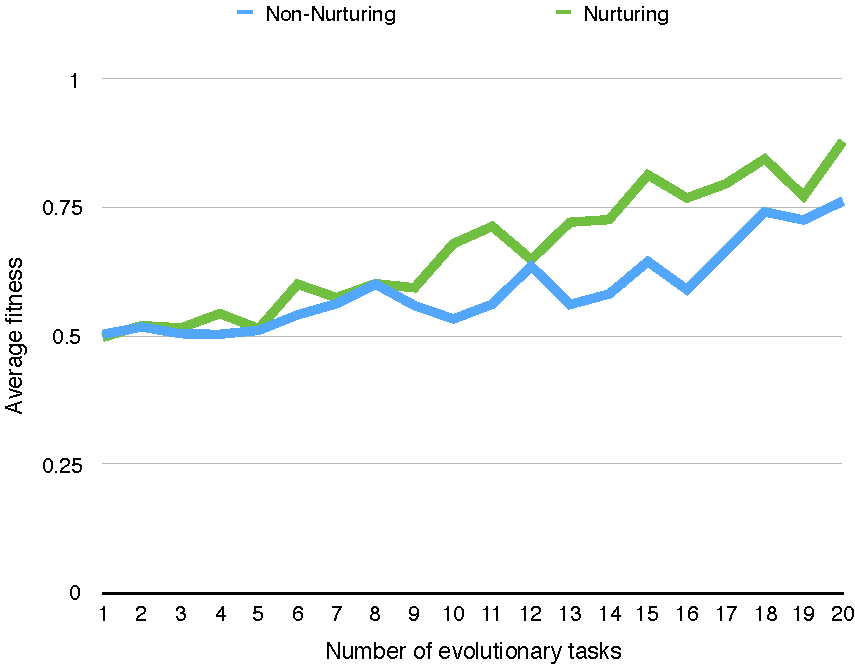
\includegraphics{NurturingGeneralizationTestPlot.pdf}
	\caption{Post-learning/nurturing generalization test on test tasks for individuals evolved under the nurturing and non-nurturing conditions.}
\end{figure}

The portion of the chromosome which encodes the learning rule is isolated and evaluated on the test tasks by initializing a network with random weights and the encoded learning rule, with the intention of determining the capacity for generalized learning that was evolved.
The differences between the results for the nurturing and non-nurturing conditions are statistically significant (randomized ANOVA, algorithm $p < 0.001$, interaction $p < 0.001$).

The linear correlation between the generalized learning fitness and the number of evolutionary tasks is statistically significant for
the intra-learning test under both the nurturing condition (Pearson correlation, $\rho=0.62,$ $p < 0.001$) 
and the non-nurturing condition (Pearson correlation, $\rho=0.43,$ $p < 0.001$)
and the post-learning test under both the nurturing condition (Pearson correlation, $\rho=0.61,$ $p < 0.001$)
and the non-nurturing condition (Pearson correlation, $\rho=0.42,$ $p < 0.001$).

Under both evaluation conditions, 
the generalized learning fitness was statistically significantly proportional to the number of evolutionary tasks,
suggesting that the quality of evolved generalized learning increases with the number of evolutionary tasks when it is also possible to evolve instincts.

In both evaluation conditions,
the learning rule evolved under the nurturing condition performed better than the learning rule evolved under the non-nurturing condition by a statistically significant margin,
suggesting that better generalized learning is expected to evolve under the nurturing condition.

$\mathbf{H_4}$: When both initial weights and learning rules are evolved, the quality of generalized learning evolved will be proportional to the number of tasks in the evolutionary environment, both with and without nurturing.

This hypothesis was supported by the results.

$\mathbf{H_6}$: When both initial weights and learning rules are evolved, higher-quality generalized learning will evolve with nurturing than without.

This hypothesis was supported by the results.

% Conclusions
\chapter{Conclusions}

%% Overall Conclusions
\section{Overall Conclusions}

The impact of varying the nurturing condition alone was insignificant; 
fitnesses measured under the nurturing condition were generally higher than those measured under the non-nurturing condition, 
but this is to be expected because of the additional fitness penalties imposed by the non-nurturing condition.

When instincts and learning were allowed to evolve alongside each other, 
it was found that instinct-based solutions were more likely to evolve for small numbers of evolutionary tasks, 
but that learning became more likely to evolve as the number of evolutionary tasks increased.

By varying the nurturing condition when instincts were allowed to evolve alongside learning, 
it was found that higher-quality generalized learning was expected to evolve under the nurturing condition than under the non-nurturing condition.

%% Contributions
\section{Contributions}

The contributions of this research are
concrete evidence that nurturing promotes the evolution of learning,
clarification of the role that instincts may play in the evolutionary process,
and a reconfirmation of Chalmers's basic conclusions \citep{Chalmers:1990aa}.

% Future Work
\chapter{Future Work}

%% The Baldwin Effect
\section{The Baldwin Effect}

Baldwin (1896) argued that learning accelerates evolution because suboptimal individuals increase their baseline fitness by acquiring more adaptive characteristics during life. 
Lifetime learning often involves a cost because the individual may be at risk at an early stage of its life or it may modify its behavior in ways that are not functional for its survival.
Baldwin suggested that evolution tends to select individuals that are born with some of the useful features that would otherwise be learned.
However, a consequence of this effect is that learned features may gradually become assimilated into the genotype and reduce the role of learning;
this is not necessarily a good effect if it is desirable for the individuals to retain the ability to learn over evolutionary time \citep{Floreano:2008wv}.

Nurturing can reduce the evolutionary costs of learning and thus may be able to inhibit the Baldwin effect.
Inhibiting the Baldwin effect may result in evolved individuals that retain greater learning capabilities over evolutionarily significant periods of time.

\bibliography{Bibliography}{}
\bibliographystyle{plainnat}

\makebackmatter
\end{document}